\documentclass{exam}
\usepackage[utf8]{inputenc}
\usepackage{lmodern}
\usepackage{microtype}

% \usepackage[parfill]{parskip}
\usepackage[dvipsnames]{xcolor}
\usepackage{amsmath}
\usepackage{amsfonts}
\usepackage{amsthm}
\usepackage{siunitx}
\DeclareSIUnit\year{yr}
\DeclareSIUnit\foot{ft}
\DeclareSIUnit\litre{\liter}

\usepackage{skull}

\usepackage{pgfplots}
\usepgfplotslibrary{polar}
\pgfplotsset{compat=1.11}
\usepgfplotslibrary{statistics}
\usepackage{graphicx}
\usepackage{sidecap}
\sidecaptionvpos{figure}{c}
\usepackage{float}
\usepackage{gensymb}
\usepackage{tkz-euclide}
\usetkzobj{all}
\usepackage{commath}
\usepackage{hyperref}
\usepackage{enumitem}
\usepackage{wasysym}
\usepackage{multicol}
\usepackage{mathtools}
\usepackage{tcolorbox}
\usepackage{tabularx}
\usepackage[version=4]{mhchem}
\usepackage{changepage}
\usepackage{listings}
\lstset{basicstyle=\ttfamily\linespread{0.8}\small}

\renewcommand*{\thefootnote}{\fnsymbol{footnote}}

\newtheorem*{thm}{Theorem}
\newtheorem*{iden}{Identity}
\newtheorem*{lemma}{Lemma}
\newtheorem{obs}{Observation}
\theoremstyle{definition}
\newtheorem*{defn}{Definition}
\newtheorem*{ex}{Example}
\newtheorem{con}{Construction}
\newtheorem*{alg}{Algorithm}

\newtheoremstyle{break}
  {\topsep}{\topsep}%
  {\itshape}{}%
  {\bfseries}{}%
  {\newline}{}%
\theoremstyle{break}
\newtheorem*{bthm}{Theorem}

% russian integral
\usepackage{scalerel}
\DeclareMathOperator*{\rint}{\scalerel*{\rotatebox{17}{$\!\int\!$}}{\int}}

% \DeclareMathOperator*{\rint}{\int}

\pgfplotsset{vasymptote/.style={
    before end axis/.append code={
        \draw[densely dashed] ({rel axis cs:0,0} -| {axis cs:#1,0})
        -- ({rel axis cs:0,1} -| {axis cs:#1,0});
    }
}}

% \pointsinrightmargin
\boxedpoints
\pointname{}

\newcommand{\questioA}{\question[\texttt{\textbf{\color{Cerulean} A}}]}
\newcommand{\questioM}{\question[\texttt{\textbf{\color{PineGreen} M}}]}
\newcommand{\questioE}{\question[\texttt{\textbf{\color{WildStrawberry} E}}]}
\newcommand{\questioS}{\question[\texttt{\textbf{\color{Goldenrod} S}}]}
\newcommand{\questioO}{\question[\texttt{\textbf{\color{BurntOrange} O}}]}

\newcommand{\parA}{\part[\texttt{\textbf{\color{Cerulean} A}}]}
\newcommand{\parM}{\part[\texttt{\textbf{\color{PineGreen} M}}]}
\newcommand{\parE}{\part[\texttt{\textbf{\color{WildStrawberry} E}}]}
\newcommand{\parS}{\part[\texttt{\textbf{\color{Goldenrod} S}}]}
\newcommand{\parO}{\part[\texttt{\textbf{\color{BurntOrange} O}}]}

\newcommand{\subparA}{\subpart[\texttt{\textbf{\color{Cerulean} A}}]}
\newcommand{\subparM}{\subpart[\texttt{\textbf{\color{PineGreen} M}}]}
\newcommand{\subparE}{\subpart[\texttt{\textbf{\color{WildStrawberry} E}}]}
\newcommand{\subparS}{\subpart[\texttt{\textbf{\color{Goldenrod} S}}]}
\newcommand{\subparO}{\subpart[\texttt{\textbf{\color{BurntOrange} O}}]}

\newcommand{\mainHeader}[2]{\section*{NCEA Level 2 Mathematics\\#1. #2}}
\newcommand{\mainHeaderHw}[2]{\section*{NCEA Level 2 Mathematics (Homework)\\#1. #2}}
\newcommand{\seealso}[1]{\begin{center}\emph{See also #1.}\end{center}}
\newcommand{\drills}[1]{\begin{center}\emph{Drill problems: #1.}\end{center}}
\newcommand{\basedon}[1]{\begin{center}\emph{Notes largely based on #1.}\end{center}}

\begin{document}

\mainHeaderDiffHw{11}{Implicit Differentiation}
\subsection*{Reading}
\begin{center}
  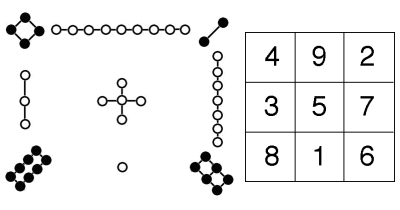
\includegraphics[width=0.5\linewidth]{chinese_magic_square}
\end{center}
Even as mathematical developments in the ancient Greek world were beginning to falter during the final centuries BCE, the burgeoning trade empire of China was leading Chinese mathematics to ever greater heights.

The simple but efficient ancient Chinese numbering system, which dates back to at least the 2nd millennium BCE, used small bamboo rods arranged to represent the numbers 1 to 9, which were then places in columns representing units, tens, hundreds, thousands, etc. It was therefore a decimal place value system, very similar to the one we use today --- indeed it was the first such number system, adopted by the Chinese over a thousand years before it was adopted in the West --- and it made even quite complex calculations very quick and easy.

Written numbers, however, employed the slightly less efficient system of using a different symbol for tens, hundreds, thousands, etc. This was largely because there was no concept or symbol of zero, and it had the effect of limiting the usefulness of the written number in Chinese.

The use of the abacus is often thought of as a Chinese idea, although some type of abacus was in use in Mesopotamia, Egypt and Greece, probably much earlier than in China (the first Chinese abacus, or ``suanpan'', we know of dates to about the 2nd Century BCE).

There was a pervasive fascination with numbers and mathematical patterns in ancient China, and different numbers were believed to have cosmic significance. In particular, magic squares --- squares of numbers where each row, column and diagonal added up to the same total --- were regarded as having great spiritual and religious significance.

The Lo Shu Square, an order three square where each row, column and diagonal adds up to 15, is perhaps the earliest of these, dating back to around 650 BCE (the legend of Emperor Yu’s discovery of the the square on the back of a turtle is set as taking place in about 2800 BCE). But soon, bigger magic squares were being constructed, with even greater magical and mathematical powers, culminating in the elaborate magic squares, circles and triangles of Yang Hui in the 13th Century (Yang Hui also produced a trianglular representation of binomial coefficients identical to the later Pascals’ Triangle, and was perhaps the first to use decimal fractions in the modern form).

But the main thrust of Chinese mathematics developed in response to the empire’s growing need for mathematically competent administrators. A textbook called ``Jiuzhang Suanshu'' or ``Nine Chapters on the Mathematical Art'' (written over a period of time from about 200 BCE onwards, probably by a variety of authors) became an important tool in the education of such a civil service, covering hundreds of problems in practical areas such as trade, taxation, engineering and the payment of wages.

It was particularly important as a guide to how to solve equations --- the deduction of an unknown number from other known information --- using a sophisticated matrix-based method which did not appear in the West until Carl Friedrich Gauss re-discovered it at the beginning of the 19th Century (and which is now known as Gaussian elimination).

Among the greatest mathematicians of ancient China was Liu Hui, who produced a detailed commentary on the ``Nine Chapters'' in 263 CE, was one of the first mathematicians known to leave roots unevaluated, giving more exact results instead of approximations. By an approximation using a regular polygon with 192 sides, he also formulated an algorithm which calculated the value of $ \pi $ as 3.14159 (correct to five decimal places), as well as developing a very early forms of both integral and differential calculus.

The Chinese went on to solve far more complex equations using far larger numbers than those outlined in the ``Nine Chapters'', though. They also started to pursue more abstract mathematical problems (although usually couched in rather artificial practical terms), including what has become known as the Chinese Remainder Theorem. This uses the remainders after dividing an unknown number by a succession of smaller numbers, such as 3, 5 and 7, in order to calculate the smallest value of the unknown number. A technique for solving such problems, initially posed by Sun Tzu in the 3rd Century CE and considered one of the jewels of mathematics, was being used to measure planetary movements by Chinese astronomers in the 6th Century AD, and even today it has practical uses, such as in Internet cryptography.

By the 13th Century, the Golden Age of Chinese mathematics, there were over 30 prestigious mathematics schools scattered across China. Perhaps the most brilliant Chinese mathematician of this time was Qin Jiushao, a rather violent and corrupt imperial administrator and warrior, who explored solutions to quadratic and even cubic equations using a method of repeated approximations very similar to that later devised in the West by Sir Isaac Newton in the 17th Century. Qin even extended his technique to solve (albeit approximately) equations involving numbers up to the power of ten, extraordinarily complex mathematics for its time.

\begin{flushright}
  From \url{http://www.storyofmathematics.com/chinese.html}.
\end{flushright}

\clearpage
\subsection*{Questions}
\begin{questions}
  \question Find $ y' $ in each case:
    \begin{parts}
      \part $ y^2 = x^3 + 3x^2 $ (Tschirnhausen cubic)
            \begin{center}
              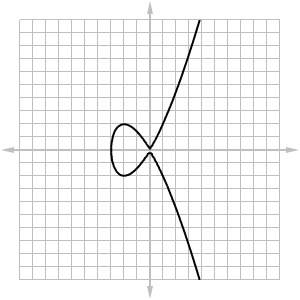
\includegraphics[width=0.3\linewidth]{implicit10}
            \end{center}
      \part $ \sin(x + y) = 2x - 2y $
            \begin{center}
              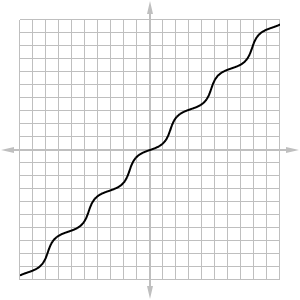
\includegraphics[width=0.3\linewidth]{implicit11}
            \end{center}
      \part $ y^2 = 5x^4 - x^2 $ (kampyle of Eudoxus)
            \begin{center}
              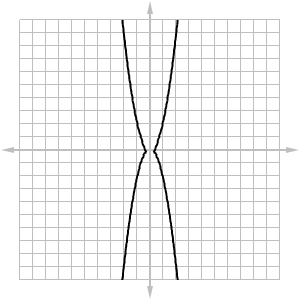
\includegraphics[width=0.3\linewidth]{implicit12}
            \end{center}
    \end{parts}
  \question Find the equation of the normal line to the curve $ x^2 + 2xy - y^2 + x = 2 $ at the point $ (1, 2) $.
  \question Show that the sum of the $ x $ and $ y $ intercepts of any tangent line to the curve $ \sqrt{x} + \sqrt{y} = \sqrt{c} $
            is just $ c $.
\end{questions}
\end{document}
